% crea il CAPITOLO
\chapter{Stato dell'arte}
% imposta l'intestazione di pagina
\lhead[\fancyplain{}{\bfseries\thepage}]{\fancyplain{}{\bfseries\rightmark}}
% mette i numeri arabi
%\pagenumbering{arabic}

In questo capitolo sono mostrati i modelli e i linguaggi utilizzati per svolgere il lavoro di tesi. Per ognuno verr\`a fatta una descrizione per esporre le caratteristiche principali ed un particolare di quelle che sono state utilizzate in questo progetto.

\section{Agenti BDI con AgentSpeak}
Il modello BDI consente di rappresentare le caratteristiche e le modalit\`a di raggiungimento di un obiettivo secondo il paradigma ad agenti. Gli agenti BDI forniscono un meccanismo per separare le attivit\`a di selezione di un piano, fra quelli presenti nella sua teoria, dall'esecuzione del piano attivo, permettendo di bilanciare il tempo speso nella scelta del piano e quello per eseguirlo.

I \textbf{beliefs} sono quindi informazioni dello stato dell'agente, ovvero ci\`o che l'agente sa del mondo: il suo insieme \`e chiamato `belief base' o `belief set'.
\\
I \textbf{desires} rappresentano tutti i possibili piani che un agente potrebbe eseguire. Rappresentano ci\`o che l'agente vorrebbe realizzare o portare a termine: i \textit{goals} sono desideri che l'agente persegue attivamente ed \`e quindi bene che tra loro siano coerenti, cosa che non \`e obbligatoria per quanto riguarda il resto dei desideri.
\\
Le \textbf{intentions} identificano i piani a cui l'agente ha deciso di lavorare o a cui sta gi\`a lavorando e a loro volta possono contenere altri piani.

Gli \textbf{eventi} innescano le attivit\`a reattive, ovvero la loro caratteristica di proattivit\`a degli agenti, come ad esempio l'aggiornamento dei beliefs, l'invocazione di piani o la modifica dei goals.

\subsection{Definizione}
\textbf{AgentSpeak} \`e un linguaggio di programmazione basato su un linguaggio del primo ordine con eventi e azioni. Il comportamento degli agenti \`e dettato da quanto definito nel programma scritto in AgentSpeak. I beliefs correnti di un agente sono relativi al suo stato attuale, l'enviroment e gli altri agenti. Gli stati che un agente vuole determinare sulla base dei suoi stimoli esterni e interni sono i desideri. L'adozione di programmi per soddisfare tali stimoli \`e detta intenzioni.

\subsection{Descrizione formale}
Vengono ora mostrate le definizioni che formalizzano questo linguaggio di programmazione.
Di seguito, nelle prime cinque definizioni, viene formalizzato il linguaggio e, nelle restanti, la semantica operazionale.

\medskip
Le specifche del linguaggio consistono in un set di beliefs e in un set di piani. Quest'ultimi sono sensibili al contesto e richiamati da eventi che permettono la scomposizione gerarchica degli obiettivi e l'esecuzione di azioni.

L'alfabeto del linguaggio formale consiste in variabili, costanti, simboli di funzione, simboli di predicati, simboli di azioni, quantificatori e simboli di punteggiatura. Oltre alle logiche del primo ordine, sono usati `!' (per achievement), `?' (per test), `;' (per operazioni sequenziali), `$\leftarrow$' (per implicazione).

\smallskip
\textbf{Definizione 1.} Se \textit{b} \`e un simbolo di predicato e \textit{t\textsubscript{1},...,t\textsubscript{n}} sono termini, allora \textit{b(t\textsubscript{1},...,t\textsubscript{n})} \`e un atomo di belief. Se \textit{b(t)} e \textit{c(s)} sono atomi di belief, allora \textit{b(t) $\land$ c(s)} e \textit{$\neg$b(t)} sono beliefs. Un atomo di belief oppure la sua negazione sono riferiti al letterale del belief.

\smallskip
\textbf{Definizione 2.} Se \textit{g} \`e un simbolo di predicato e \textit{t\textsubscript{1},...,t\textsubscript{n}} sono termini, allora !\textit{g(t\textsubscript{1},...,t\textsubscript{n})} e ?\textit{g(t\textsubscript{1},...,t\textsubscript{n})} sono \textit{goals}.

\smallskip
\textbf{Definizione 3.} Se \textit{b}(t) \`e un atomo di belief , !\textit{g(t)} e ?\textit{g(t)} sono goals, allora +\textit{b(t)}, -\textit{b(t)}, +!\textit{g(t)}, -!\textit{g(t)}, +?\textit{g(t)}, -?\textit{g(t)} sono \textit{eventi di attivazione}.

\smallskip
\textbf{Definizione 4.} Se \textit{a} \`e un simbolo di azione e \textit{t\textsubscript{1},...,t\textsubscript{n}} sono termini del primo ordine, allora \textit{a(t\textsubscript{1},...,t\textsubscript{n})} \`e un'azione.

\smallskip
\textbf{Definizione 5.} Se \textit{e} \`e un evento scatenante, \textit{b\textsubscript{1},...,b\textsubscript{n}} sono letterali di belief e \textit{h\textsubscript{1};...;h\textsubscript{n}} sono goals o azioni, allora \textit{e : b\textsubscript{1}$\land$...$\land$b\textsubscript{m} $\leftarrow$ h\textsubscript{1};...;h\textsubscript{n}} \`e un piano.

\bigskip
Durante l'esecuzione un agente \`e composto di un set di beliefs B, un set di piani P, un set di intenzioni I, un set di eventi E, un set di azioni A e un set di funzioni di selezione S, il quale \`e formato da S\textsubscript{E} (funzione di selezione degli eventi), S\textsubscript{O} (funzione di selezione del piano), S\textsubscript{I} (funzione di selezione dell'intenzione).

\smallskip
\textbf{Definizione 6.} Un \textit{agente} \`e formato da $\langle$E,B,P,I,A,\textit{S\textsubscript{E},S\textsubscript{O},S\textsubscript{I}}$\rangle$, dove E \`e un set di eventi, B \`e una 'belief base', P \`e un set di piani, I \`e un set di intenzioni, A \`e un set di azioni. La funzione \textit{S\textsubscript{E}} sceglie un evento da E; la funzione \textit{S\textsubscript{O}} sceglie un piano dal set di quelli applicabili; la funzione \textit{S\textsubscript{I}} sceglie l'intenzione da eseguire da I.

\smallskip
\textbf{Definizione 7.} Il set I \`e composto da intenzioni, ognuna delle quali \`e una pila di piani parzialmente istanziati (dove alcune variabili sono state istanziate). Un'intenzione \`e definita da [\textit{p\textsubscript{1}$\ddagger$...$\ddagger$p\textsubscript{z}}], dove \textit{p\textsubscript{1}} \`e il fondo dello stack e \textit{p\textsubscript{z}} la testa. Gli elementi sono delimitati da $\ddagger$. Per convenienza [+!true:true $\leftarrow$ true] \`e detta \textit{true intention} e viene definita con T.

\smallskip
\textbf{Definizione 8.} Il set E \`e composto da eventi, oguno delle quali \`e una tupla \textit{$\langle$\textit{e}, \textit{i}$\rangle$}, dove \textit{e} \`e l'evento e \textit{i} un'intenzione. Se l'intenzione \`e di tipo \textit{true intention} allora dove \textit{e} sar\`a chiamato \textit{evento esterno}, altrimenti \`e un \textit{evento interno}.

\smallskip
\textbf{Definizione 9.} Sia \textit{S\textsubscript{E}}(E) = \textit{$\epsilon$} = $\langle$\textit{d}, \textit{i}$\rangle$ e sia \textit{p} = \textit{e : b\textsubscript{1}$\land$...$\land$b\textsubscript{m} $\leftarrow$ h\textsubscript{1};...;h\textsubscript{n}}, il piano \textit{p} \`e rilevante per l'evento \textit{e} se e solo se esiste un unificatore $\sigma$ tale per cui d$\sigma$ = e$\sigma$. \textit{$\sigma$} \`e detto \textit{unificatore rilevante} per \textit{$\epsilon$}.

\smallskip
\textbf{Definizione 10.} Un piano \textit{p} \`e definito da \textit{e : b\textsubscript{1}$\land$...$\land$b\textsubscript{m} $\leftarrow$ h\textsubscript{1};...;h\textsubscript{n}} \`e un \textit{piano applicabile} rispetto ad un evento \textit{e} se e solo se esite un identificatore rilevante $\sigma$ per \textit{$\epsilon$} e esite una sostituzione \textit{$\theta$} tale che $\forall$\textit{(b\textsubscript{1}$\land$...$\land$b\textsubscript{m})}\textit{$\sigma\theta$} \`e una conseguenza logica di B. La composizione \textit{$\sigma\theta$} \`e riferita all'\textit{unificatore applicabile} per l'evento \textit{$\epsilon$} e \textit{$\theta$} \`e riferita alla sostituzione della corretta risposta.


\smallskip
\textbf{Definizione 11.} Sia S\textsubscript{O}(O\textsubscript{\textit{$\epsilon$}}) = \textit{p}, dove O\textsubscript{\textit{$\epsilon$}} \`e il set dei piani applicabili per l'evento \textit{$\epsilon$} =$\langle$\textit{d}, \textit{i}$\rangle$ e \textit{p} \`e \textit{e : b\textsubscript{1}$\land$...$\land$b\textsubscript{m} $\leftarrow$ h\textsubscript{1};...;h\textsubscript{n}}. Il piano \textit{p} \`e destinato all'evento \textit{$\epsilon$}, dove \textit{i} \`e la \textit{true intention} se e solo se esiste un \textit{unificatore applicabile} \textit{$\sigma$} per cui [+!true:true $\leftarrow$ true $\ddagger$ (\textit{e : b\textsubscript{1}$\land$...$\land$b\textsubscript{m} $\leftarrow$ h\textsubscript{1};...;h\textsubscript{n}})$\sigma$ ] $\in$ I.

\smallskip
\textbf{Definizione 12.} Sia S\textsubscript{O}(O\textsubscript{\textit{$\epsilon$}}) = \textit{p}, dove O\textsubscript{\textit{$\epsilon$}} \`e il set dei piani applicabili per l'evento \textit{$\epsilon$} = $\langle$\textit{d}, [\textit{p\textsubscript{1}} $\ddagger$ ... $\ddagger$ \textit{f} : c\textsubscript{1}$\land$...$\land$c\textsubscript{y} $\leftarrow$ !\textit{g(t)};h\textsubscript{2};...;h\textsubscript{n}]$\rangle$, e \textit{p} \`e +!\textit{g(s)} : b\textsubscript{1}$\land$...$\land$b\textsubscript{m} $\leftarrow$ k\textsubscript{1};...;k\textsubscript{j}. Il piano \textit{p} \`e destinato all'evento \textit{$\epsilon$} se e solo se esiste un \textit{unificatore applicabile} \textit{$\sigma$} tale che [\textit{p\textsubscript{1}} $\ddagger$ ... $\ddagger$ \textit{f} : c\textsubscript{1}$\land$...$\land$c\textsubscript{y} $\leftarrow$ !\textit{g(t)};h\textsubscript{2};...;h\textsubscript{n} $\ddagger$ (
+!\textit{g(s)} : b\textsubscript{1}$\land$...$\land$b\textsubscript{m}) $\sigma$ $\leftarrow$ (k\textsubscript{1};...;k\textsubscript{j}) $\sigma$; (h\textsubscript{2};...;h\textsubscript{n})$\sigma$] $\in$ I.

\smallskip
\textbf{Definizione 13.} Sia S\textsubscript{I}(I) = \textit{i}, dove \textit{i} \`e [\textit{p\textsubscript{1}} $\ddagger$ ... $\ddagger$ \textit{f} : c\textsubscript{1}$\land$...$\land$c\textsubscript{y} $\leftarrow$ !\textit{g(t)};h\textsubscript{2};...;h\textsubscript{n}]. L'intenzione \textit{i} si dice che \`e eseguita  se e solo se $\langle$ +!\textit{g(t)}, \textit{i} $\rangle$ $\in$ E.

\smallskip
\textbf{Definizione 14.} Sia S\textsubscript{I}(I) = \textit{i}, dove \textit{i} \`e [\textit{p\textsubscript{1}} $\ddagger$ ... $\ddagger$ \textit{f} : c\textsubscript{1}$\land$...$\land$c\textsubscript{y} $\leftarrow$ ?\textit{g(t)};h\textsubscript{2};...;h\textsubscript{n}]. L'intenzione \textit{i} si dice che \`e eseguita  se e solo se esiste una sostituzione \textit{$\theta$} tale che $\forall$g(t)\textit{$\theta$} \`e una conseguenza logica di B e \textit{i} \`e rimpiazzato da [\textit{p\textsubscript{1}} $\ddagger$ ... $\ddagger$ (\textit{f} : c\textsubscript{1}$\land$...$\land$c\textsubscript{y})\textit{$\theta$} $\leftarrow$ h\textsubscript{2}\textit{$\theta$};...;h\textsubscript{n}\textit{$\theta$}].

\smallskip
\textbf{Definizione 15.} Sia S\textsubscript{I}(I) = \textit{i}, dove \textit{i} \`e [\textit{p\textsubscript{1}} $\ddagger$ ... $\ddagger$ \textit{f} : c\textsubscript{1}$\land$...$\land$c\textsubscript{y} $\leftarrow$ \textit{a(t)};h\textsubscript{2};...;h\textsubscript{n}]. L'intenzione \textit{i} si dice che \`e eseguita  se e solo se \textit{a(t)} $\in$ A, e \textit{i} \`e rimpiazzato da [\textit{p\textsubscript{1}} $\ddagger$ ... $\ddagger$ \textit{f} : c\textsubscript{1}$\land$...$\land$c\textsubscript{y} $\leftarrow$ h\textsubscript{2};...;h\textsubscript{n}].

\smallskip
\textbf{Definizione 16.} Sia S\textsubscript{I}(I) = \textit{i}, dove \textit{i} \`e [\textit{p\textsubscript{1}} $\ddagger$ ... $\ddagger$ \textit{p\textsubscript{z-1}} $\ddagger$ \textit{g(t)} : c\textsubscript{1}$\land$...$\land$c\textsubscript{y} $\leftarrow$ \textit{true}], dove \textit{p\textsubscript{z-1}} \`e e : b\textsubscript{1}$\land$...$\land$b\textsubscript{x} $\leftarrow$ !\textit{g(s)}; h\textsubscript{2};...;h\textsubscript{n}. L'intenzione \textit{i} si dice che \`e eseguita  se e solo se esiste una sostituzione \textit{$\theta$} tale che g(t)\textit{$\theta$} = g(s)\textit{$\theta$} e \textit{i} \`e rimpiazzato da [\textit{p\textsubscript{1}} $\ddagger$ ... $\ddagger$ \textit{p\textsubscript{z-1}} $\ddagger$ (e : b\textsubscript{1}$\land$...$\land$b\textsubscript{x})textit{$\theta$} $\leftarrow$ (h\textsubscript{2}\textit{$\theta$};...;h\textsubscript{n})\textit{$\theta$}].



\subsubsection{Ciclo di ragionamento}
Il ciclo di ragionamento \`e il modo in cui l'agente prende le sue decisioni e mette in pratica le azioni. Esso \`e composto di otto fasi: le prime tre sono quelle che riguardano l'aggiornamento dei belief relativi al mondo e agli altri agenti, mentre altre descrivono la selezione di un evento che permette l'esecuzione di un'intenzione dell'agente.

%/---AGGIORNAMENTO BELIEF BASE---/
\subsubsection{a. Percezione ambiente}
La percezione effettuata dall'agente all'interno del ciclo di ragionamento \`e utilizzata per poter aggiornare il suo stato. L'agente interroga dei componenti capaci di rilevare i cambiamenti nell'ambiente e di emettere dati consultabili utilizzando opportune interfacce.

\subsubsection{b. Aggiornamento beliefs}
Ottenuta la lista delle percezioni \`e necessario aggiornare la `belief base'. Ogni percezione non ancora presente nel set viene aggiunta e al contrario quelle presenti nel set e che non sono nella lista delle percezioni vengono rimosse.
Ogni cambiamento effettato nella `belief base' produce un evento: quelli generati da percezioni dell'ambiente sono detti eventi esterni; quelli interni, rispetto agli altri, hanno associata un'intenzione.

\subsubsection{c. Ricezione e selezione messaggi}
L'altra sorgente di informazioni per un agente sono gli altri agenti presenti nel sistema. L'interprete controlla i messaggi diretti all'agente e li rende a lui disponibili: ad ogni iterazione del ciclo pu\`o essere processato solo un messaggio. Inoltre,pu\`o essere assegnata una priotit\`a ai messaggi in coda definendo una funzione di prelazione per l'agente.
\\
Prima di essere processati i messaggi passano all'interno di una funzione di selezione che definisce quali messaggi possano essere accettati dall'agente. Questa funzione pu\`o essere implementata ad esempio per far ricevere solo i messaggi un certo agente.

%/---SELEZIONE EVENTO E ESECUZIONE INTENZIONE---/
\subsubsection{d. Selezione evento}
Gli eventi rappresentano la percezione del cambiamento nell'ambiente o dello stato interno dell'agente, come il goal. Ci possono essere vari eventi in attesa ma in ogni ciclo di ragionamento pu\`o esserne gestito uno solo, il quale viene scelto dalla funzione di selezione degli eventi che ne seleziona uno dalla lista di quelli in attesa. Se la lista di eventi fosse vuota si passa direttamente alla penultima fase del ciclo di ragionamento, ovvero la selezione di un'intenzione.

\subsubsection{e. Recupero piani rilevanti}
Una volta selezionato l'evento \`e necessario trovare un piano che permetta all'agente di agire per gestirlo. Per fare ci\`o viene recuperata dalla `Plan Library' la lista dei piani rilevanti, verificando quali possano essere unificati con l'evento selezionato. L'unificazione \`e il confronto relativo a predicati e termini. Al termine di questa fase si otterr\`a un set di piani rilevanti per l'evento selezionato che verr\`a raffinato successivamente.

\subsubsection{f. Selezione piano appplicabile}
Ogni piano ha un contesto che definisce con quali informazioni dell'agente pu\`o essere usato.
Per piano applicabile si intendeno quelli che, in relazione allo stato dell'agente, possono avere una possibilit\`a di successo. Viene quindi controllato che il contesto sia una conseguenza logica della `belief base' dell'agente. Vi possono anche essere pi\`u piani in grado di gestire un evento ma l'agente deve selezionarne uno solo ed impegnarsi ad eseguirlo.
\\La selezione viene fatta tramite un'apposita funzione che inoltre tiene conto dell'ordinamento dei piani in base alla loro posizione nel codice sorgente oppure dall'ordine di inserimento. Quando un piano \`e scelto, viene creata un'istanza di quel piano che viene inserita nel set delle intenzioni: sar\`a l'istanza ad essere manipolata dall'interprete e non il piano nella libreria.

Ci sono due possibili modalit\`a per la creazione di un'intenzione e dipende dal fatto che l'evento selezionato sia esterno o interno. Nel primo caso viene semplicemente creata l'intenzione, altrimenti viene inserita un'altra intenzione in testa a quella che ha generato l'evento, poich\`e \`e necessario eseguire fino al completamento un piano per raggiungere tale goal.

\subsubsection{g. Selezione intenzione}
A questo punto, se erano presenti eventi da gestire, \`e stata aggiunta un'altra intenzione nello stack. Un agente ha tipicamente pi\`u di un'intenzione nel set delle intenzioni che potrebbe essere eseguita, ognuna delle quali rappresenta un diverso punto di attenzione. Ad ogni ciclo di ragionamento avviene l'esecuzione di una sola intenzione, la cui scelta \`e importante per come l'agente operer\`a nell'ambiente.

\subsubsection{h. Esecuzione intenzione}
L'intenzione, scelta nello step precedente, non \`e altro che il corpo di un piano formato da una sequenza di istruzioni, ognuna delle quali, una volta eseguita, viene rimossa dall'istanza del piano. Terminata l'esecuzione un'intenzione, quest'ultima viene restituita al set delle intenzioni a meno che non debba aspettare un messaggio o un feedback dell'azione: in questo caso viene memorizzata in una struttura e restituita una volta ricevuta la risposta.
Se un'intenzione \`e sospesa non pu\`o essere selezionata per l'esecuzione nel ciclo di ragionamento.

\subsubsection{Scambio di messaggi}
Lo scambio di messaggi \`e la comunicazione standard che avviene tra agenti per comunicare tra loro e operare in base al contenuto ricevuto.
La comunicazione definita da AgentSpeak utilizza tre parti. La prima \`e la coda dei messaggi in input, ovvero una lista contenente tutti i messaggi che il sistema o interprete riceve e che sono destinati all'agente. La seconda \`e la coda dei messaggi di output che si allunga ogni volta che l'agente vuole inviare un messaggio ad un altro agente. L'ultima \`e una struttura all'interno della quale vengono memorizzate le intenzioni che sono sospese dall'esecuzione poich\`e aspettano una risposta dal canale di comunicazione dei messaggi.
\\
L'interprete \`e il mezzo per il quale i messaggi trasmessi. Esso infatti ha il compito di recuperare tutti i messaggi nella coda in uscita di ogni agente e successivamente recapitarli. Per la consegna viene recuperato l'agente destinatario di ogni messaggio e poi quest'ultimo viene posizionato nella coda di quelli in input dell'agente, in modo tale che possa recuperarne il contenuto al prossimo ciclo di ragionamento.

\section{Caratteristiche Jason}
Jason \`e la maggiore implementazione di AgentSpeak e, oltre ad implementare le sue semantiche operazionali, lo estende dichiarando il linguaggio per definire gli agenti. Jason aggiunge un set di meccanismi potenti per migliorare le abilit\`a degli agenti ed, inoltre, mira a rendere pi\`u pratico il linguaggio di programmazione ad agenti. Alcuni dei meccanismi aggiunti da Jason sono:
\begin{itemize}
\item negazione forte;
\item gestione del fallimento dei piani;
\item atti linguistici basati sulla comunicazione inter-agente;
\item annotazioni sulle etichette del piano che possono essere utilizzate mediante funzioni di selezione elaborate;
\item supporto per gli ambienti di sviluppo;
\item possibilit\`a di eseguire un sistema multi-agente distribuito su una rete;
\item funzioni di selezione personalizzabili, funzioni di trust, architettura generale dell'agente;
\item estensibilit\`a mediante azioni interne definite dall'utente.
\end{itemize}

%----------------------------
\section{tuProlog}
tuProlog \`e un interprete Prolog per le applicazioni e le infrastrutture Internet basato su Java. \`E progettato per essere facilmente utilizzabile, leggero, configurabile dinamicamente, direttamente integrato in Java e facilmente interoperabile.
tuProlog \`e sviluppato e mantenuto da `aliCE' un gruppo di ricerca dell'Alma Mater Studiorum - Universit\`a di Bologna, sede di Cesena. \`E un software Open Source e rilasciato sotto licenza LGPL.

\subsection{Caratteristiche tuProlog}
tuProlog ha diverse caratteristiche e qui di seguito verranno illustrate solo alcune di esse, ovvero quelle utilizzate all'interno di questo lavoro.
Il motore tuProlog fornisce e riconosce i seguenti tipi di predicati:
\begin{itemize}
\item predicati built-in: incapsulati nel motore tuProlog;
\item predicati di libreria: inseriti in una libreria che viene caricata nel motore tuProlog. La libreria pu\`o essere liberamente aggiunta all'inizio o rimossa dinamicamente durante l'esecuzione. I predicati della libreria possono essere sovrascritti da quelli della teoria. Per rimuovere un singolo predicato dal motore \`e necesssario rimuovere tutta la libreria che contiene quel predicato;
\item predicati della teoria: inseriti in una teoria che viene caricata nel motore tuProlog. Le teorie tuProlog sono semplicemente collezioni di clausole Prolog. Le teorie possono essere liberamente aggiunte all'inizio o rimosse dinamicamente durante l'esecuzione.
\end{itemize}

In questo lavoro \`e stato utilizzato il motore tuProlog, fornito tramite la libreria Java `alice.tuprolog', e le funzionalit\`a collegate per monitorare e modificare la teoria di ogni agente.

Una peculiare modalit\`a di utilizzo di tuProlog sfruttata in questo progetto \`e stata la registrazione di oggetti Java all'interno della teoria dell'agente. In questo modo \`e possibile utilizzare uno stesso oggetto sia nella parte Java che in quella tuProlog. Nello specifico, come verr\`a mostrato nella parte relativa all'implementazione, questa funzionalit\`a \`e stata utilizzata per registrare la classe stessa dell'agente in tuProlog e consentendo l'invocazione di metodi implementati lato Java direttamente dalla teoria dell'agente.

%----------------------------
\section{Alchemist}
Alchemist \`e un simulatore per il calcolo pervasivo, aggregato e ispirato alla natura. Esso fornisce un ambiente di simulazione sul quale \`e possibile sviluppare nuove incarnazioni, cio\`e nuove definizioni di modelli implementati su di esso. Ad oggi sono disponibili le funzionalit\`a per:
\begin{itemize}
\item simulare un ambiente bidimensionale;
\item simulare mappe del mondo reale, con supporto alla navigazione e importazione di tracciati in formato gpx;
\item simulare ambienti indoor importando immagini in bianco e nero;
\item eseguire simulazioni biologiche utilizzando reazioni in stile chimico;
\item eseguire programmi Protelis, Scafi, SAPERE (scritti in un linguaggio basato su tuple come LINDA).
\end{itemize}

\subsection{Meta-modello}
Il meta-modello di Alchemist pu\`o essere compreso osservando la figura \ref{fig:alchemistModel}.
%crea l'ambiente figura;
\begin{figure}[h] % [h] sta per here, cioè la figura va qui
\begin{center} % centra nel mezzo della pagina la figura
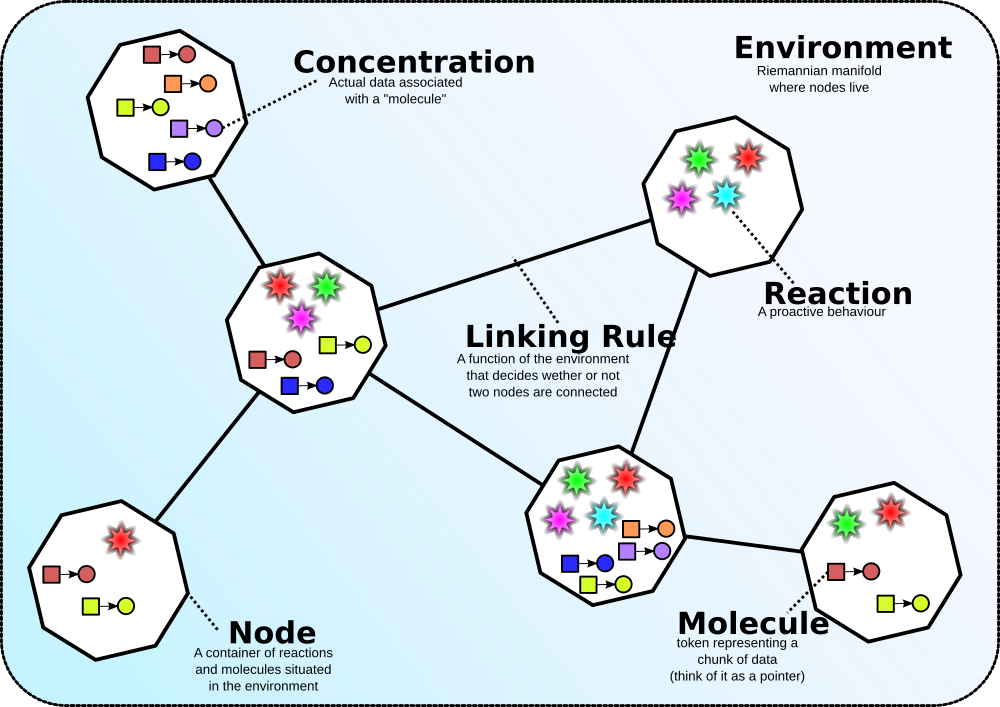
\includegraphics[width=12.5cm]{images/AlchemistModel.png} % inserisce una figura larga 12.5cm
% inserisce la legenda ed etichetta la figura con \label{fig:prima}
\caption[Illustrazione meta-modello di Alchemist]{Illustrazione meta-modello di Alchemist} \label{fig:alchemistModel}
\end{center}
\end{figure}

L'\textbf{\textit{Environment}} \`e l'astrazione dello spazio ed \`e anche l'entit\`a pi\`u esterna che funge da contenitore per i nodi. Conosce la posizione di ogni nodo nello spazio ed \`e quindi in grado di fornire la distanza tra due di essi e ne permette inoltre lo spostamento.

\`E detta \textbf{\textit{Linking rule}} una funzione dello stato corrente dell'environemnt che associa ad ogni nodo un \textbf{\textit{Vicinato}}, il quale \`e un entit\`a composta da un nodo centrale e da un set di nodi vicini.

Un \textbf{\textit{Nodo}} \`e un contenitore di molecole e reazioni che \`e posizionato all'interno di un environment.

La \textbf{\textit{Molecola}} \`e il nome di un dato, paragonabile a quello che rappresenta il nome di una variabile per i linguaggi imperativi.
Il valore da associare ad una molecola \`e detto \textbf{\textit{Concentrazione}}.

%crea l'ambiente figura;
\begin{figure}[h] % [h] sta per here, cioè la figura va qui
\begin{center} % centra nel mezzo della pagina la figura
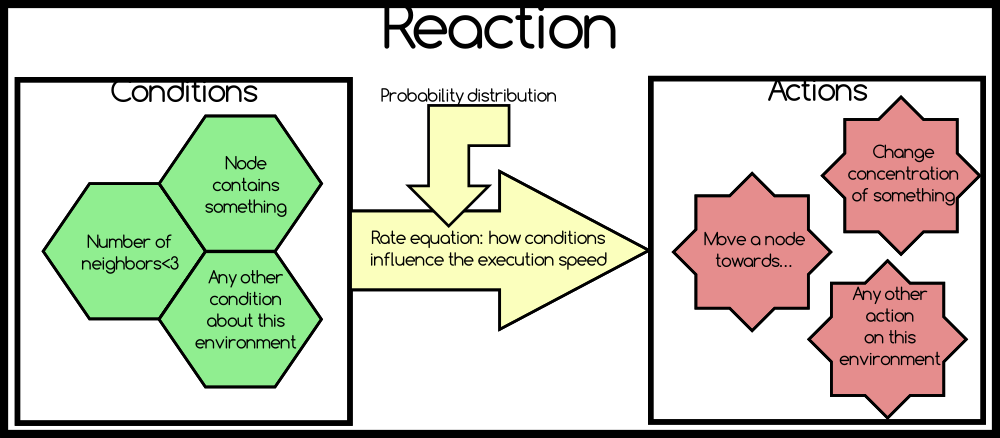
\includegraphics[width=14cm]{images/AlchemistReaction.png} % inserisce una figura larga 12.5cm
% inserisce la legenda ed etichetta la figura con \label{fig:prima}
\caption[Illustrazione modello reazione di Alchemist]{Illustrazione modello reazione di Alchemist} \label{fig:alchemistReaction}
\end{center}
\end{figure}

Una \textbf{\textit{Reazione}} \`e un qualsiasi evento che pu\`o cambiare lo stato dell'environment ed \`e definita tramite una distribuzione temporale, una lista di condizioni e una o pi\`u azioni.
\\La frequenza con cui avvengono dipende da:
\begin{itemize}
\item un parametro statico di frequenza;
\item il valore di ogni condizione;
\item un'equazione di frequenza che combina il parametro statico e il valore delle condizioni restituendo la frequenza istantanea;
\item una distribuzione temporale.
\end{itemize}
Ogni nodo contiene un set di reazioni che pu\`o essere anche vuoto.

Per comprendere meglio il meccanismo di una reazione si pu\`o osservare la figura \ref{fig:alchemistReaction}.

Una \textbf{\textit{Condizione}} \`e una funzione che prende come input l'environment corrente e restituisce come output un booleano e un numero. Se la condizione non si verifica, le azioni associate a quella reazione non saranno eseguite. In relazione a parametri di configurazione e alla distribuzione temporale, una condizione potrebbe influire sulla velocit\`a della reazione.

La \textbf{\textit{Distribuzione temporale}} indica il numero di eventi, in un dato intervallo di tempo, generati da Alchemist e che innescano la verifica delle condizioni che possono portare alla potenziale esecuzione delle azioni.

Un'\textbf{\textit{Azione}} \`e la definizione di una serie di operazioni che modellano un cambiamento nel nodo o nell'environment.

In Alchemist un'incarnazione \`e un'istanza concreta del meta-modello appena descritta e che implementa una serie di componenti base come: la definizione di una molecola e del tipo di dati della concentrazione, un set di condizioni, le azioni e le reazioni. Incarnazioni diverse possono modellare universi completamente differenti.

\subsection{Esempi (?)}


%----------------------------
\section{LINDA}
LINDA \`e un modello di coordinazione e comunicazione tra diversi processi paralleli che operano su oggetti immagazzinati e recuperati dalla memoria associativa, virtuale, condivisa. Nel modello diverse primitive operano su una sequenza ordinata di oggetti, le `tuple', che vengono aggiunte ad un linguaggio sequenziale e una memoria associativa logica globale, detta spazio di tuple, nel quale i processi immagazzinano e recuperano le tuple.

Il modello LINDA originale definisce quattro operazioni consentite sulle tuple e lo spazio di tuple:
\begin{itemize}
\item \textit{in}: legge una tupla e la consuma dallo spazio di tuple
\item \textit{rd}: legge una tupla senza consumarla dallo spazio di tuple
\item \textit{out}: inserisce una tupla nello spazio di tuple
\item \textit{eval}: crea un processo per valutare le tuple e lo inserisce nello spazio di tuple.
\end{itemize}

LINDA \`e un modello di coordinazione utilizzato per definire altri modelli e tecnologie di coordinazione, dove gli agenti distribuiti interagiscono e si coordinano tramite scambio di messaggi utilizzando spazi di informazione condivisa e sfruttando la comunicazione generativa.

La sintassi del processo di calcolo in LINDA \`e definito tramite la seguente grammatica:
\\
\textit{P, Q ::= t |} outeval\textit{(P).Q} | rd\textit{(t).P} | in\textit{(t).P} | \textit{P + Q} | rec\textit{X.P} | \textit{X}

Di seguito \`e descritta un'estensione del modello appena descritto chiamata Spatial Tuples dove le informazioni base assumono una posizione e un'estensione nello spazio fisico.

\subsection{Spatial Tuples}
Spatial Tuples \`e un estensione del modello base di tuple per i sistemi distribuiti multi-agente, dove
\begin{itemize}
\item le tuple sono posizionate nel mondo fisico e si possono muovere;
\item il comportamento delle primitive di coordinamento pu\`o dipendere dalle propriet\`a spaziali del coordinamento degli agenti;
\item lo spazio di tuple pu\`o essere concepito come un livello virtuale che aumenta la realt\`a fisica.
\end{itemize}
Spatial Tuples supporta esplicitamente la consapevolezza dello spazio e la coordinazione basata sullo spazio dell'agente in scenari di calcolo pervasivo.

Questo modello pu\`o risultare molto utile in scenari dove gli utenti si spostano all'interno di un ambiente fisico aumentato e devono coordinarsi con altri utenti, che siano persone o agenti.

\subsubsection{Modello e linguaggio}
Spatial Tuples si occupa prima di tutto di tuple spaziali. Una tupla spaziale \`e una tupla associata ad un'informazione spaziale. Le informazioni spaziali possono essere, ad esempio, GPS, amministrative, organizzative: in ogni caso la tupla viene associata a qualche luogo o regione dello spazio fisico.
\\
Una tupla spaziale decora lo spazio fisico e pu\`o funzionare come meccanismo base per aumentare la realt\`a con informazioni di ogni sorta. Una volta che la tupla \`e associata ad una regione o posizione, le sue informazioni possono essere pensate come propriet\`a attribuite a quella porzione di spazio fisico. Accedendo alle tuple con i meccanismi di Spatial Tuples, l'informazione pu\`o essere osservata da qualsiasi agente che si occupa dello spazio fisico specifico in modo tale da comportarsi di conseguenza.
\\
Inoltre, una tupla pu\`o essere associata anche ad un componente situato. In questo caso, se il componente cambia la sua posizione nel tempo, finch\`e non viene rimossa, anche la tupla si sposter\`a con esso.

In Spatial Tuples viene introdotto un linguaggio di descrizione dello spazio per specificare le informazioni spaziali che decorano le truple. Questo linguaggio \`e ortogonale al linguaggio di comunicazione e ha lo scopo di fornire l'ontologia di base che definisce i concetti spaziali.

\subsubsection{Primitive spaziali}
Gli operatori base di Spatial Tuples sono: \textbf{out(t)}, \textbf{rd(tt)}, \textbf{in(tt)} dove t \`e la tupla e tt \`e un template di tupla. Il funzionamento delle primitive \`e il seguente:
\begin{itemize}
\item \textit{out}, permette di associare la tupla ad una regione o posizione;
\item \textit{rd}, cerca le tuple che corrispondono al template e ne ritorna una copia;
\item \textit{in}, come rd, cerca le tuple che corrispondo al template ma poi ne restituisce una consumandola dalla sorgente.
\end{itemize}
Le primitive \textit{rd} e \textit{out} sono dette `getter' e, in Spatial Tuples, sono: 
\begin{itemize}
\item sospensive, se non ci sono tuple che fanno match con il template l'operazione \`e bloccata finch\`e non viene trovata una tupla
\item non deterministiche, se vi sono pi\`u tuple che fanno match con il template una \`e scelta in modo non deterministico.
\end{itemize}

%--------------------------------------
%Le caratteristiche di un agente sono:
%\begin{itemize}
%	\item Autonomia
%	\item Reattivit\`a
%	\item Proattivit\`a
%	\item Orientamento ai goal
%	\item Socialit\`a
%	\item Adatattivit\`a
%	\item Cognitivit\`a
%\end{itemize}